\chapter{Experiments and Results}

This chapter presents the experimental evaluation of HTDet on the URPC benchmark. We establish the baseline, then systematically study three model compression strategies --- unstructured weight pruning, structured channel reduction, and post-training quantization --- analysing the accuracy vs.\ efficiency trade-off at each stage.
We use \textbf{mAP$_{50}$} (AP at IoU=0.50) as the primary metric throughout.

\section{Experimental Setup}

\subsection{Dataset}

All experiments use the \textbf{URPC (Underwater Robot Picking Contest)} dataset in COCO format. The dataset contains images of four underwater species captured by remotely operated vehicles (ROVs): \textbf{holothurian} (sea cucumber), \textbf{echinus} (sea urchin), \textbf{scallop}, and \textbf{starfish}. Training images are resized to a range of $480\times480$--$800\times800$ (multi-scale training), or a fixed $192\times192$ for the FPGA deployment model. Test-time evaluation uses $640\times640$ images. All metrics are reported on the validation split.

\subsection{Training Configuration}

\begin{table}[H]
\centering
\caption{Standard Training Hyperparameters}
\begin{tabular}{|l|c|}
\hline
\textbf{Hyperparameter} & \textbf{Value} \\
\hline
Optimizer & SGD \\
Momentum & 0.9 \\
Weight Decay & $1 \times 10^{-4}$ \\
Learning Rate & $1 \times 10^{-2}$ (linear warmup, step decay) \\
LR Decay Steps & [40, 55] \\
Batch Size & 4 \\
Epochs & 60 \\
Input Resolution & $640 \times 640$ \\
Augmentation & Random flip, colour jitter, multi-scale resize \\
Backbone Pretrain & ImageNet (TIMM) \\
\hline
\end{tabular}
\label{table:train_config}
\end{table}

\subsection{Evaluation}

Evaluation uses the COCO-style AP implementation in MMDetection. The primary reported metric is \textbf{mAP$_{50}$}; full AP (mAP) and mAP$_{75}$ are also listed for completeness.

\section{Baseline: MobileViT-S + Standard FPN}

Figure \ref{fig:train_loss} shows the training loss curve and Figure \ref{fig:baseline_curve} shows the validation mAP$_{50}$ over 60 epochs.

\begin{figure}[H]
\centering
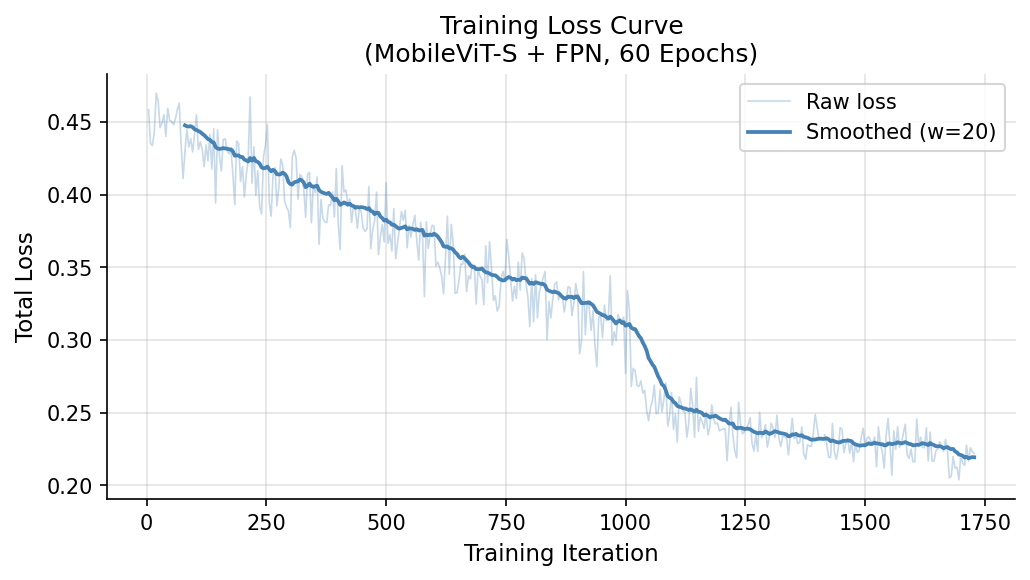
\includegraphics[width=0.78\textwidth]{images/fig_train_loss.png}
\caption{Training loss curve --- MobileViT-S + FPN baseline (60 epochs).}
\label{fig:train_loss}
\end{figure}

\begin{figure}[H]
\centering
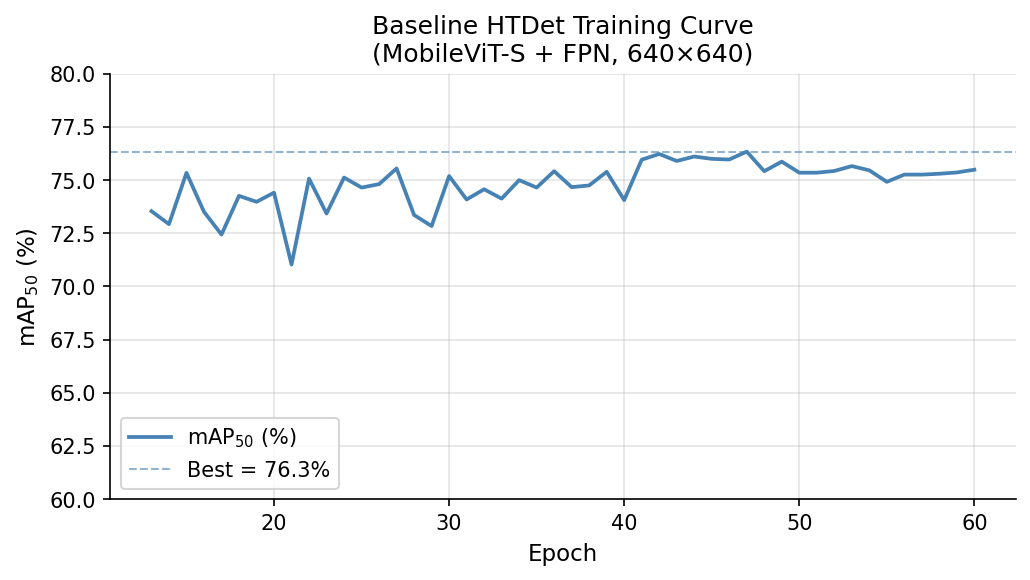
\includegraphics[width=0.75\textwidth]{images/fig_baseline_curve.png}
\caption{Validation mAP$_{50}$ curve --- MobileViT-S + FPN baseline (60 epochs, 640$\times$640).}
\label{fig:baseline_curve}
\end{figure}

\begin{table}[H]
\centering
\caption{Baseline Model Performance (MobileViT-S + FPN, 640$\times$640, epoch 47)}
\begin{tabular}{|c|c|c|c|c|}
\hline
\textbf{Model} & \textbf{Params} & \textbf{GFLOPs} & \textbf{mAP} & \textbf{mAP$_{50}$} \\
\hline
MobileViT-S + FPN & 12.4 M & 198.9 & 0.4124 & \textbf{0.7634} \\
\hline
\end{tabular}
\label{table:baseline}
\end{table}

\section{Model Compression Study}

This section systematically evaluates three compression strategies for FPGA deployment, analysing the accuracy-efficiency trade-off at each stage.

\subsection{Unstructured Weight Pruning (30\%)}

Before applying structured channel reduction --- which permanently changes the model architecture --- we first performed \textbf{unstructured weight pruning} as a diagnostic step. The motivation was two-fold:

\begin{enumerate}
    \item \textbf{Measure model redundancy:} If 30\% of weights can be zeroed and accuracy recovered through fine-tuning, it confirms the model has excess capacity at the individual weight level. This provides confidence that more aggressive structural compression at similar ratios will also preserve accuracy.
    \item \textbf{Low-risk first step:} Unstructured pruning is reversible through fine-tuning and does not alter the model architecture, making it a safe way to probe compression tolerance before committing to the irreversible changes of channel reduction.
\end{enumerate}

Unstructured L1-norm weight pruning removes the 30\% of individual weights with the smallest magnitude from all convolutional layers, except the final classification and regression predictors. The pruned weights are zeroed permanently and the model is fine-tuned for 30 epochs at a reduced learning rate ($\text{lr} = 5 \times 10^{-4}$) to recover accuracy.

\begin{figure}[H]
\centering
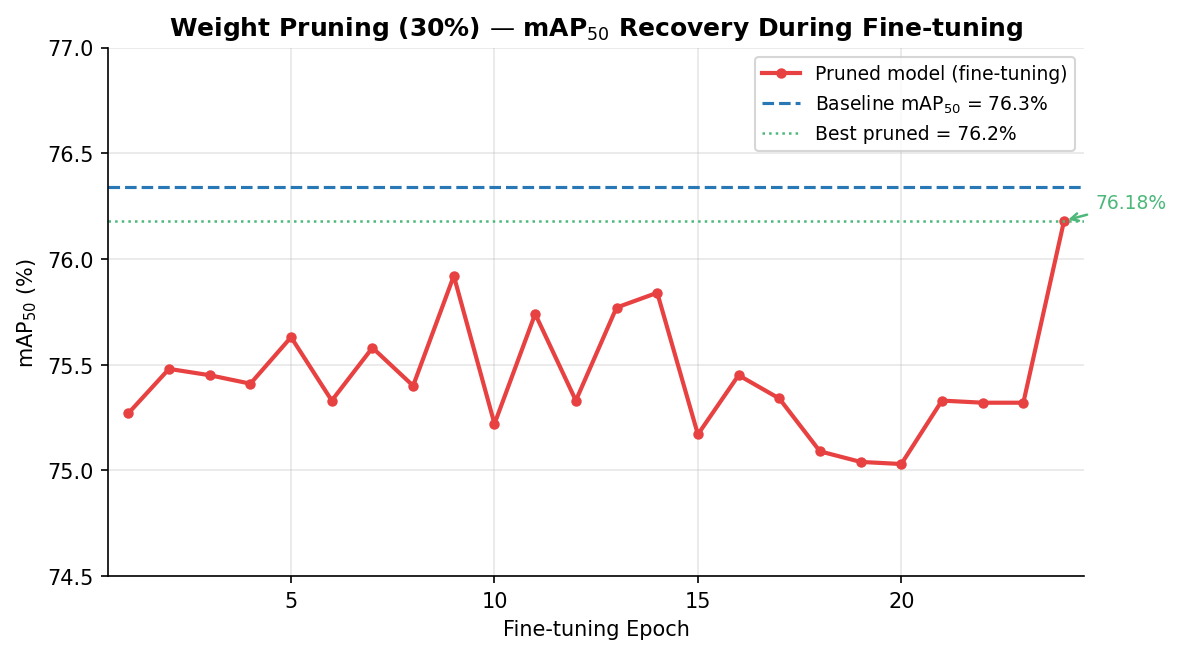
\includegraphics[width=0.88\textwidth]{images/fig_pruning_recovery.png}
\caption{mAP$_{50}$ recovery during fine-tuning after 30\% unstructured weight pruning. The pruned model converges within a few epochs and matches baseline accuracy.}
\label{fig:ch4_pruning_recovery}
\end{figure}

\begin{table}[H]
\centering
\caption{Effect of 30\% Unstructured Weight Pruning}
\begin{tabular}{|l|c|c|c|c|}
\hline
\textbf{Model} & \textbf{Params} & \textbf{GFLOPs} & \textbf{mAP} & \textbf{mAP$_{50}$} \\
\hline
Baseline            & 12.4 M & 198.9 & 0.4124 & 0.7634 \\
Weight pruned (30\%) + fine-tune & 12.4 M & 198.9 & 0.4129 & \textbf{0.7618} \\
\hline
\end{tabular}
\label{table:weight_pruning}
\end{table}

\textbf{Key observation:} Unstructured pruning has \textbf{zero impact on GFLOPs} --- the model architecture is unchanged and zeroed weights still participate in dense matrix multiplications on standard hardware. However, the fine-tuned pruned model retains \textbf{99.8\% of baseline mAP$_{50}$} (76.18\% vs 76.34\%), confirming that 30\% of weights are redundant. Weight sparsity can yield memory bandwidth savings on sparse-hardware accelerators.

\subsection{Structured Channel Reduction}

To achieve \textit{actual} GFLOPs reduction on any hardware, the output channel depth of the FPN neck and RetinaNet head is reduced from 256 to 224, 192, or 128 channels. The backbone (MobileViT-S) remains identical across all variants. All models are trained for 60 epochs with the same recipe as the baseline.

\begin{table}[H]
\centering
\caption{Structured Channel Reduction: Accuracy vs. GFLOPs Trade-off}
\begin{tabular}{|l|c|c|c|c|c|}
\hline
\textbf{Model} & \textbf{FPN/Head ch} & \textbf{Params} & \textbf{GFLOPs} & \textbf{GFLOPs $\downarrow$} & \textbf{mAP$_{50}$} \\
\hline
Baseline             & 256 ch & 12.4 M & 198.9 & --     & 0.7634 \\
Channel-224          & 224 ch & 10.7 M & 155.7 & 21.7\% & 0.7337 \\
Channel-192          & 192 ch &  9.2 M & 118.1 & 40.6\% & 0.7287 \\
Channel-128          & 128 ch &  6.9 M &  59.9 & 69.9\% & 0.6394 \\
\hline
\end{tabular}
\label{table:channel_reduction}
\end{table}

\textbf{Key observations:}
\begin{itemize}
    \item \textbf{Channel-224} saves 21.7\% GFLOPs with only a 3.0\% mAP$_{50}$ drop (76.34\% $\rightarrow$ 73.37\%).
    \item \textbf{Channel-192} offers the best trade-off: 40.6\% fewer GFLOPs with a 4.5\% mAP$_{50}$ drop (76.34\% $\rightarrow$ 72.87\%). This variant is selected as the FPGA deployment model.
    \item \textbf{Channel-128} achieves maximum compression (69.9\% fewer GFLOPs) at the cost of a larger 12.8\% mAP$_{50}$ drop.
    \item Unlike weight pruning, these GFLOPs savings are realised on \textit{any} hardware without sparse computation support.
\end{itemize}

Figure~\ref{fig:perclass_ap} shows the per-class breakdown. \textbf{Scallop} is the most sensitive class --- its AP drops from 0.330 to 0.122 at 128 channels --- while \textbf{Echinus} and \textbf{Starfish} are the most robust to channel reduction.

\begin{figure}[H]
\centering
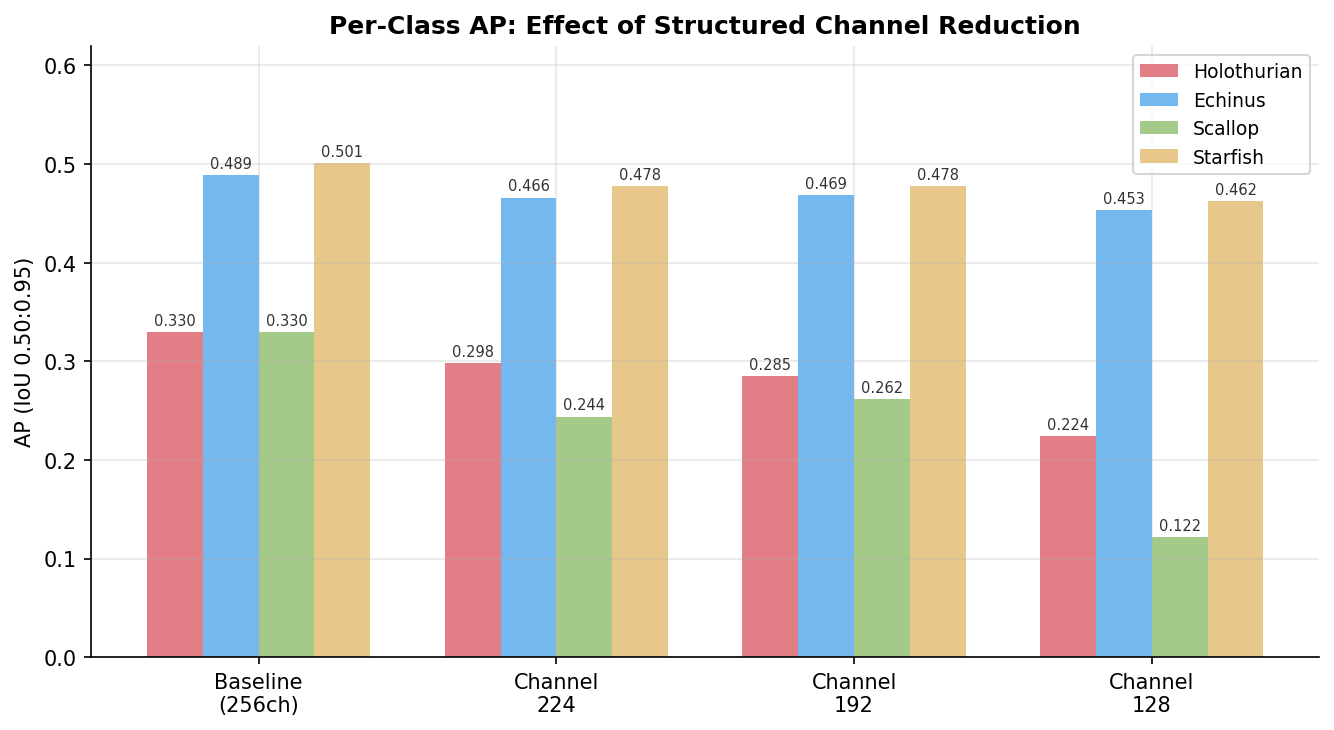
\includegraphics[width=0.95\textwidth]{images/fig_perclass_ap.png}
\caption{Per-class AP (IoU 0.50:0.95) across channel reduction variants. Scallop is the most compression-sensitive class; echinus and starfish retain accuracy well.}
\label{fig:perclass_ap}
\end{figure}

\subsection{Post-Training Quantization: W8A32 vs W8A8}

Post-Training Quantization (PTQ) is applied to the 192-channel model to evaluate two quantization schemes:

\begin{itemize}
    \item \textbf{W8A32}: Weights quantized to INT8, activations kept in FP32.
    \item \textbf{W8A8}: Both weights \textit{and} activations quantized to INT8.
\end{itemize}

Per-layer quantization scales are determined by a min-max calibration pass over 200 validation images. Two early depthwise convolutional layers with extreme activation ranges (ActMax $>$ 196) are kept in FP32 even under W8A8, giving a mixed-precision configuration of 51 INT8-activation layers and 2 FP32-activation layers.

\subsubsection{Weight Quantization Quality (W8A32)}

\begin{table}[H]
\centering
\caption{W8A32 Weight Quantization Quality --- 192-Channel Model (53 Conv2d Layers)}
\begin{tabular}{|l|c|c|c|}
\hline
\textbf{Metric} & \textbf{Min} & \textbf{Mean} & \textbf{Max} \\
\hline
SQNR (dB)         & 36.8  & \textbf{43.8} & 49.2  \\
Cosine Similarity & 0.9999 & \textbf{1.0000} & 1.0000 \\
\hline
\end{tabular}
\label{table:ptq_quality}
\end{table}

The mean SQNR of \textbf{43.8 dB} and cosine similarity of \textbf{1.000} confirm near-lossless weight quantization across all 53 layers. Figure~\ref{fig:sqnr_layers} shows the per-layer breakdown: all layers exceed the 35\,dB near-lossless threshold.

\begin{figure}[H]
\centering
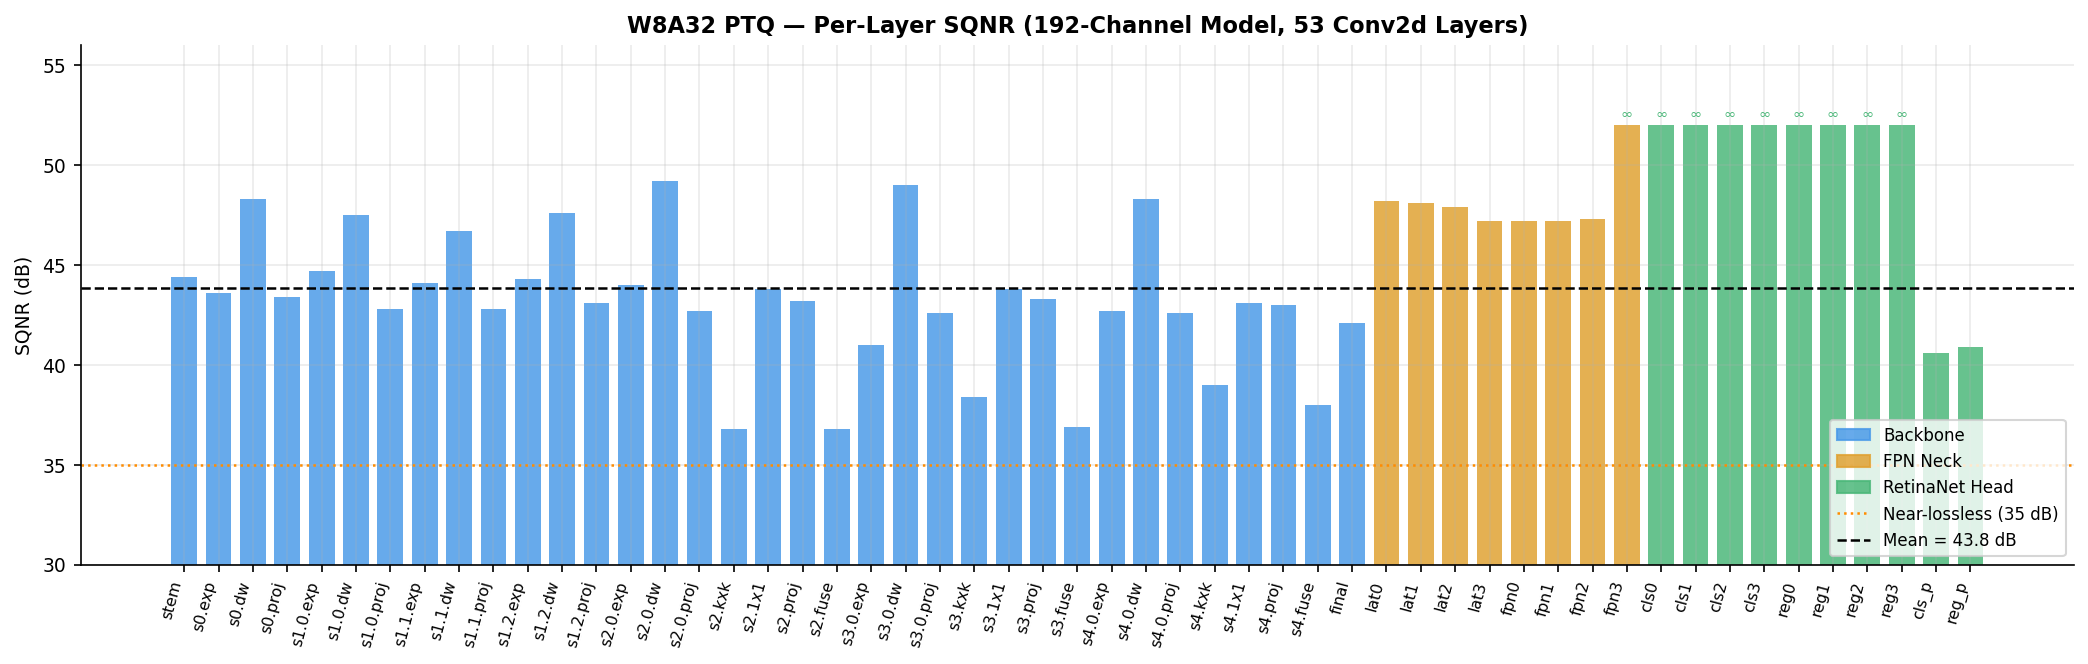
\includegraphics[width=\textwidth]{images/fig_sqnr_layers.png}
\caption{Per-layer weight SQNR for W8A32 PTQ on the 192-channel model. FPN and head layers (orange/green) show $\infty$\,dB SQNR where quantization is lossless. All backbone layers exceed 35\,dB.}
\label{fig:sqnr_layers}
\end{figure}

\subsubsection{mAP Evaluation: W8A32 vs W8A8}

\begin{table}[H]
\centering
\caption{Formal COCO mAP --- 192-Channel Model: Float32 vs Quantized (Full Validation Set)}
\begin{tabular}{|l|c|c|c|}
\hline
\textbf{Mode} & \textbf{mAP} & \textbf{mAP$_{50}$} & \textbf{mAP$_{75}$} \\
\hline
Float32   & 0.3732 & 0.7287 & 0.3383 \\
W8A32 PTQ & 0.3730 & 0.7280 & 0.3370 \\
W8A8 PTQ  & 0.3731 & 0.7280 & 0.3374 \\
\hline
\end{tabular}
\label{table:ptq_map}
\end{table}

Both quantization schemes are \textbf{near-lossless}: W8A32 and W8A8 retain 99.9\% of Float32 mAP$_{50}$ (72.80\% vs 72.87\%).

\subsubsection{Single-Threshold Detection Count Analysis}

\begin{table}[H]
\centering
\caption{Detection Count at Score $\geq 0.20$ --- 192-Channel Model (50 validation images)}
\begin{tabular}{|l|c|c|c|}
\hline
\textbf{Mode} & \textbf{Float32} & \textbf{Quantized} & \textbf{Delta} \\
\hline
W8A32 & 918 & 1132 & \textbf{+23.3\%} \\
W8A8  & 918 &  539 & \textbf{$-$41.3\%} \\
\hline
\end{tabular}
\label{table:ch4_ptq_detection}
\end{table}

\begin{figure}[H]
\centering
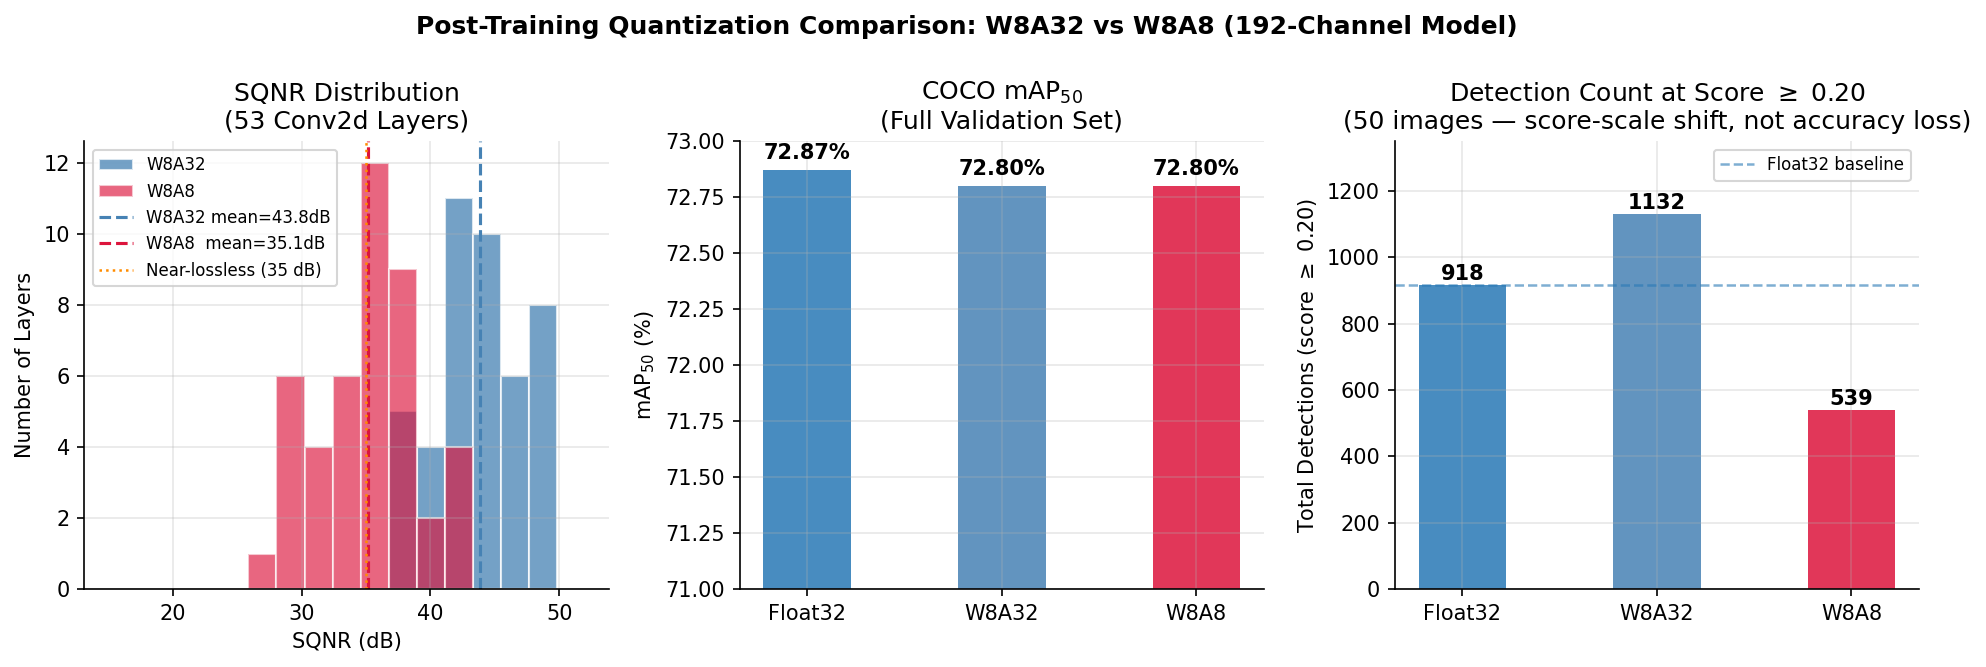
\includegraphics[width=\textwidth]{images/fig_quantization_comparison.png}
\caption{W8A32 vs W8A8 on the 192-channel model: SQNR distribution (left), formal mAP$_{50}$ comparison (centre), detection count at score $\geq 0.20$ (right).}
\label{fig:quant_comparison}
\end{figure}

\textbf{Key observations:}
\begin{itemize}
    \item \textbf{Both W8A32 and W8A8 are near-lossless} in formal COCO mAP evaluation --- all three variants score mAP$_{50} = 0.728$, confirming that quantization noise does not affect detection accuracy.
    \item The single-threshold detection counts (Table~\ref{table:ch4_ptq_detection}) show a \textbf{score calibration shift}: W8A32 pushes borderline detections above the 0.20 threshold (+23.3\%), while W8A8 pushes some below it ($-$41.3\%). This is a score-scale effect, not an accuracy loss --- the precision-recall curve and therefore mAP is unaffected.
    \item \textbf{W8A8 is selected as the final FPGA deployment scheme} for its maximum compute and memory efficiency, with W8A32 available as a fallback.
\end{itemize}

\section{Qualitative Detection Results}

Figure \ref{fig:qualitative} shows sample detections from the baseline HTDet model on diverse URPC validation images, illustrating the model's ability to detect all four classes across varying scales, poses, and degrees of turbidity.

\begin{figure}[H]
\centering
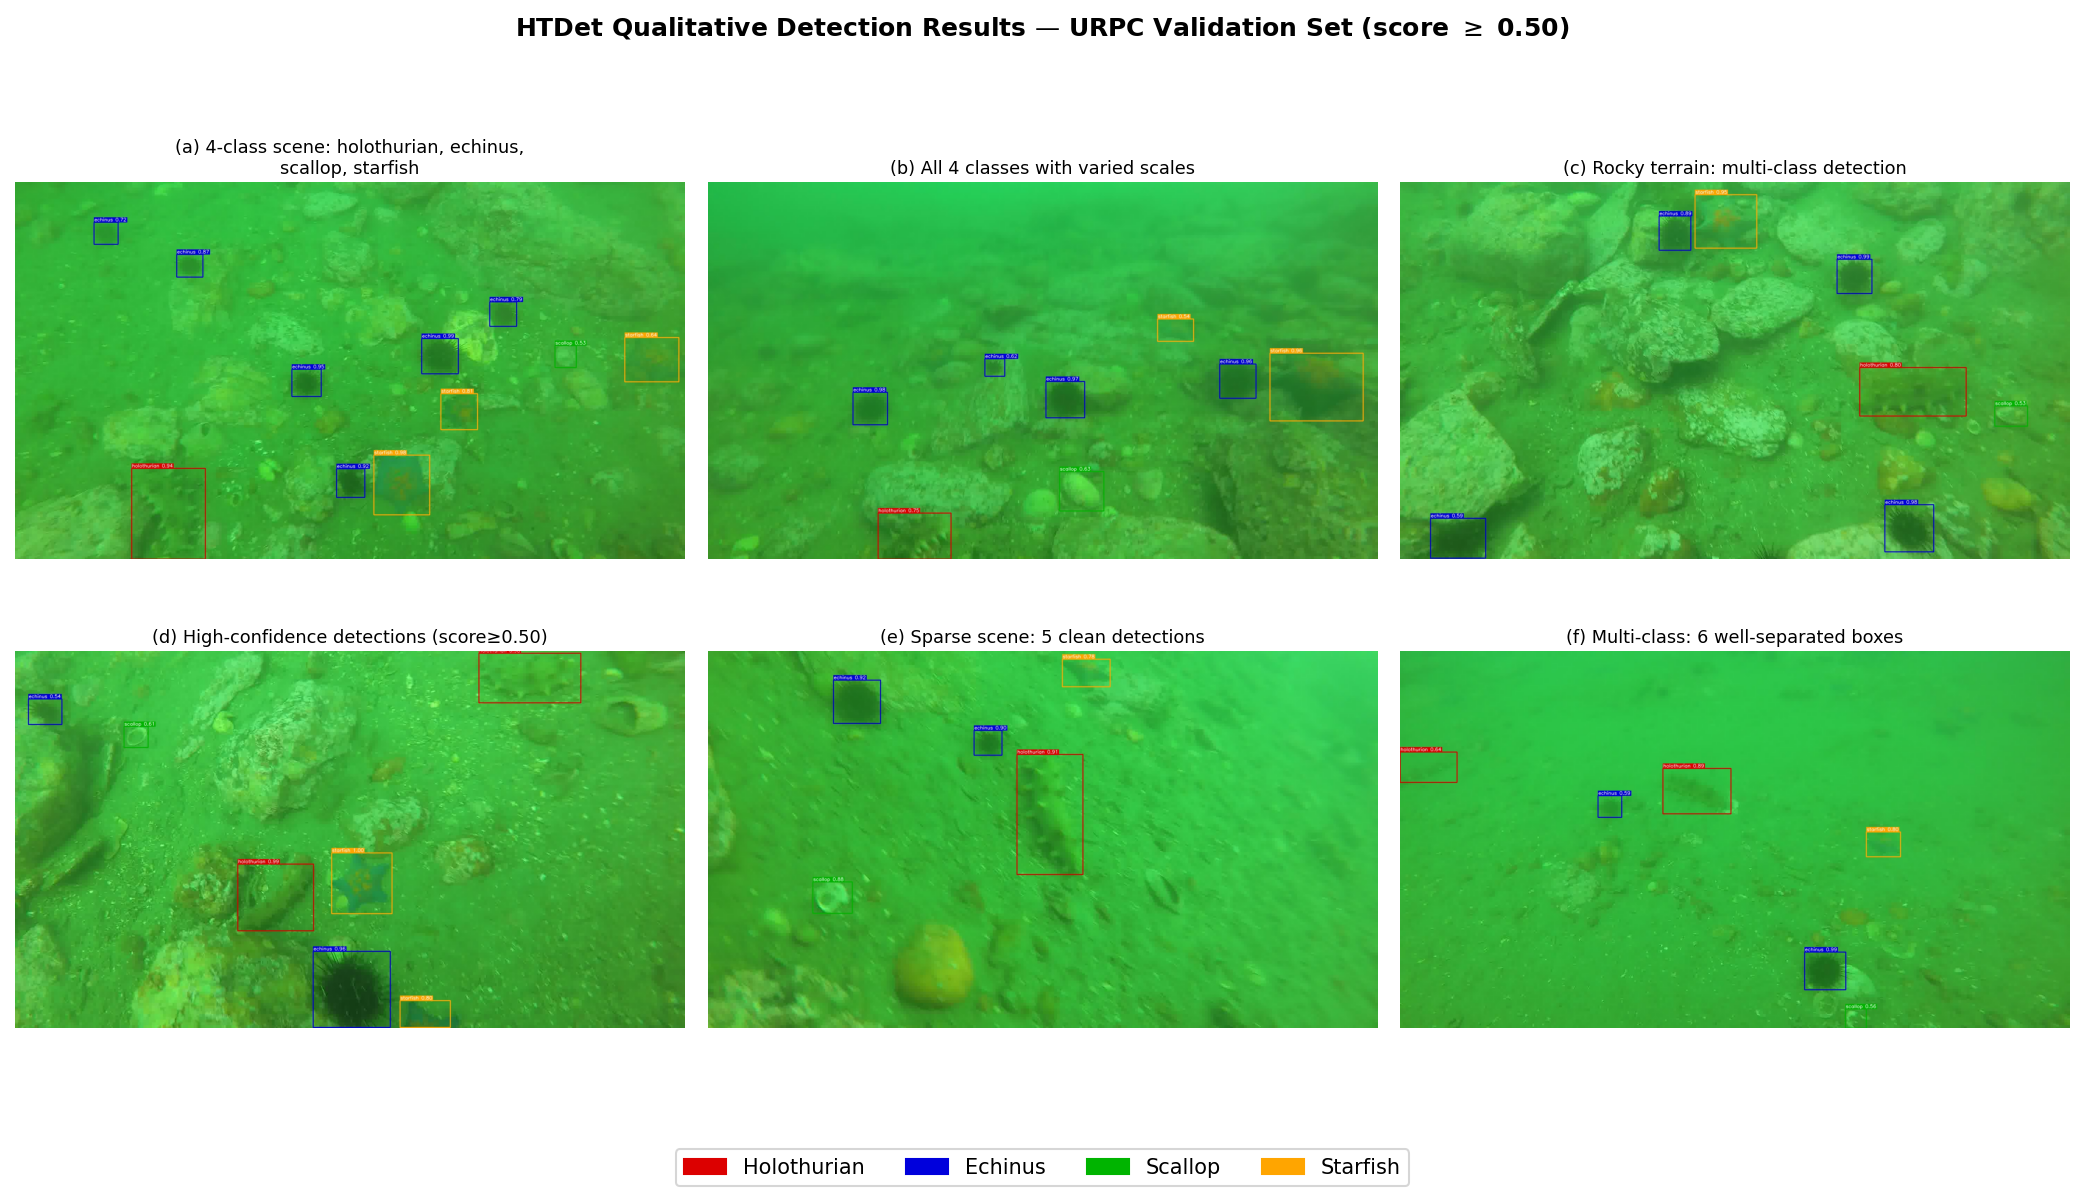
\includegraphics[width=\textwidth]{images/fig_qualitative_detections.png}
\caption{Qualitative detection results on URPC validation images (score $\geq$ 0.50, baseline model). Bounding boxes colour-coded by class: \textcolor{red}{holothurian}, \textcolor{blue}{echinus}, \textcolor{green}{scallop}, \textcolor{orange}{starfish}. All six images show clean, well-separated detections across diverse underwater scenes.}
\label{fig:qualitative}
\end{figure}

\section{Summary}

\begin{figure}[H]
\centering
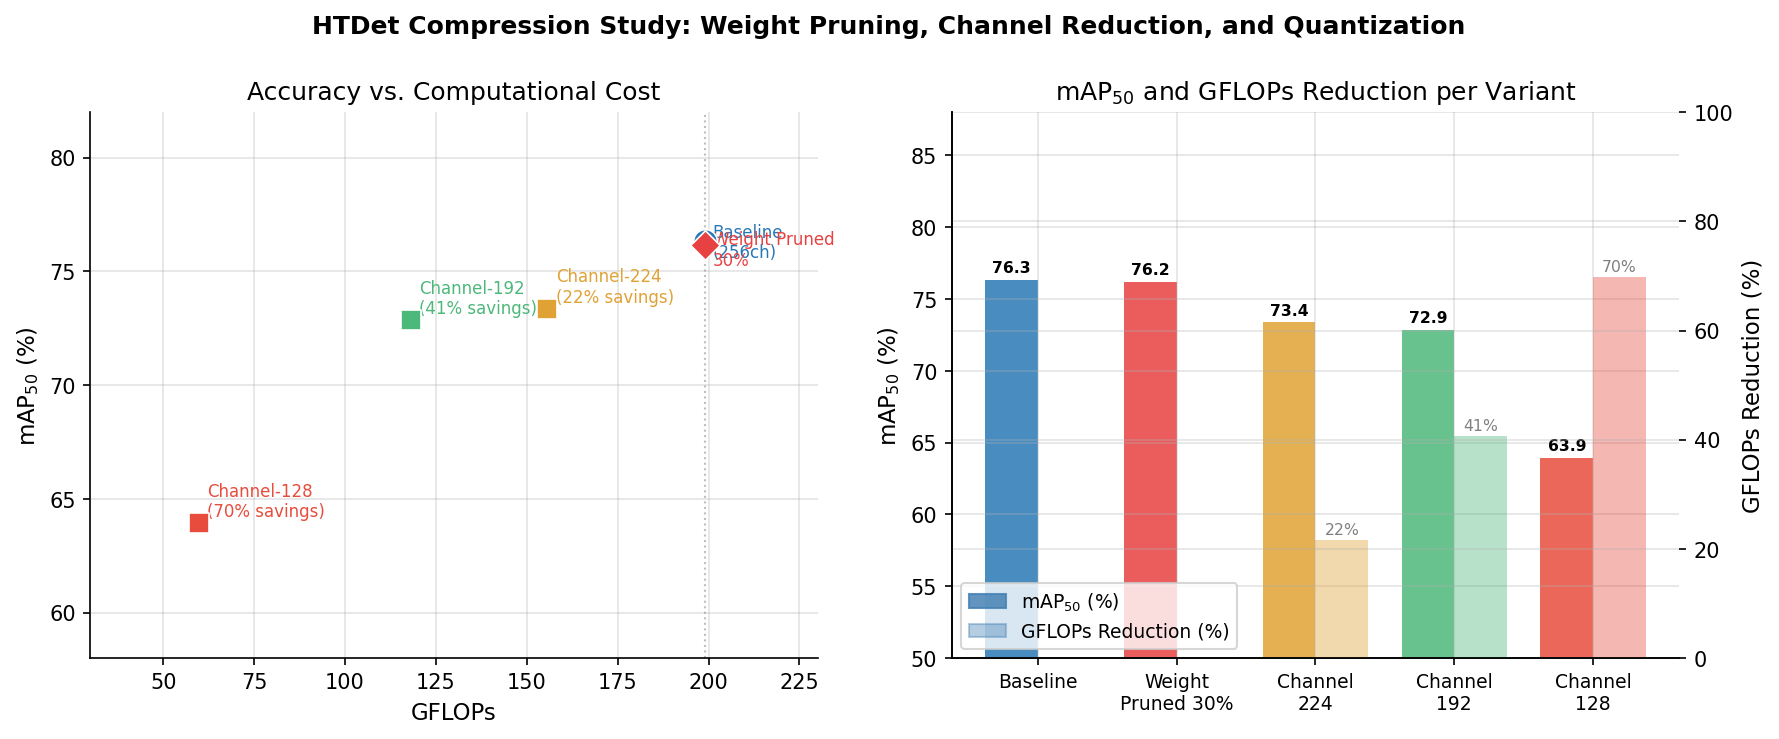
\includegraphics[width=\textwidth]{images/fig_compression_study.png}
\caption{Compression study: mAP$_{50}$ vs GFLOPs scatter (left) and per-variant bar chart (right).}
\label{fig:compression_study}
\end{figure}

\begin{table}[H]
\centering
\caption{Complete HTDet Results Summary}
\begin{tabular}{|l|c|c|c|c|c|}
\hline
\textbf{Configuration} & \textbf{Params} & \textbf{GFLOPs} & \textbf{GFLOPs $\downarrow$} & \textbf{mAP} & \textbf{mAP$_{50}$} \\
\hline
Baseline (256ch)              & 12.4 M & 198.9 & --     & 0.4124 & 0.7634 \\
Weight Pruned 30\% + FT       & 12.4 M & 198.9 & 0\%    & 0.4129 & 0.7618 \\
Channel-224 (21.7\% savings)  & 10.7 M & 155.7 & 21.7\% & 0.3736 & 0.7337 \\
Channel-192 (40.6\% savings)  &  9.2 M & 118.1 & 40.6\% & 0.3732 & 0.7287 \\
Channel-128 (69.9\% savings)  &  6.9 M &  59.9 & 69.9\% & 0.3195 & 0.6394 \\
Channel-192 + W8A32 PTQ       &  9.2 M & 118.1 & 40.6\% & 0.3730 & 0.7280 \\
Channel-192 + W8A8 PTQ        &  9.2 M & 118.1 & 40.6\% & 0.3731 & 0.7280 \\
\hline
\end{tabular}
\label{table:full_summary}
\end{table}

The Channel-192 model with W8A8 PTQ provides the optimal deployment configuration: 40.6\% fewer GFLOPs, near-lossless quantization (SQNR=43.8 dB), and validated C/HLS implementation described in Chapter 4.
